\section*{Experimental Results}

The dataset used for the experiments is the famous \emph{Recipes1M+} \cite{15}, a collection 
created by MIT, consisting of more than one million culinary recipes. 
Of all these recipes, only a subset of 51235 documents of it was used due 
to their informative content which best fits the purpose of this study. The 
information about the line distributions for each recipe indicates that the 
instruction field contains a higher number than the information contained in 
the ingredients field. To have good performance in finding, we preferred to 
choose the "instructions" field (\ref{distributions}).

\begin{figure}[h!]
    \centering
    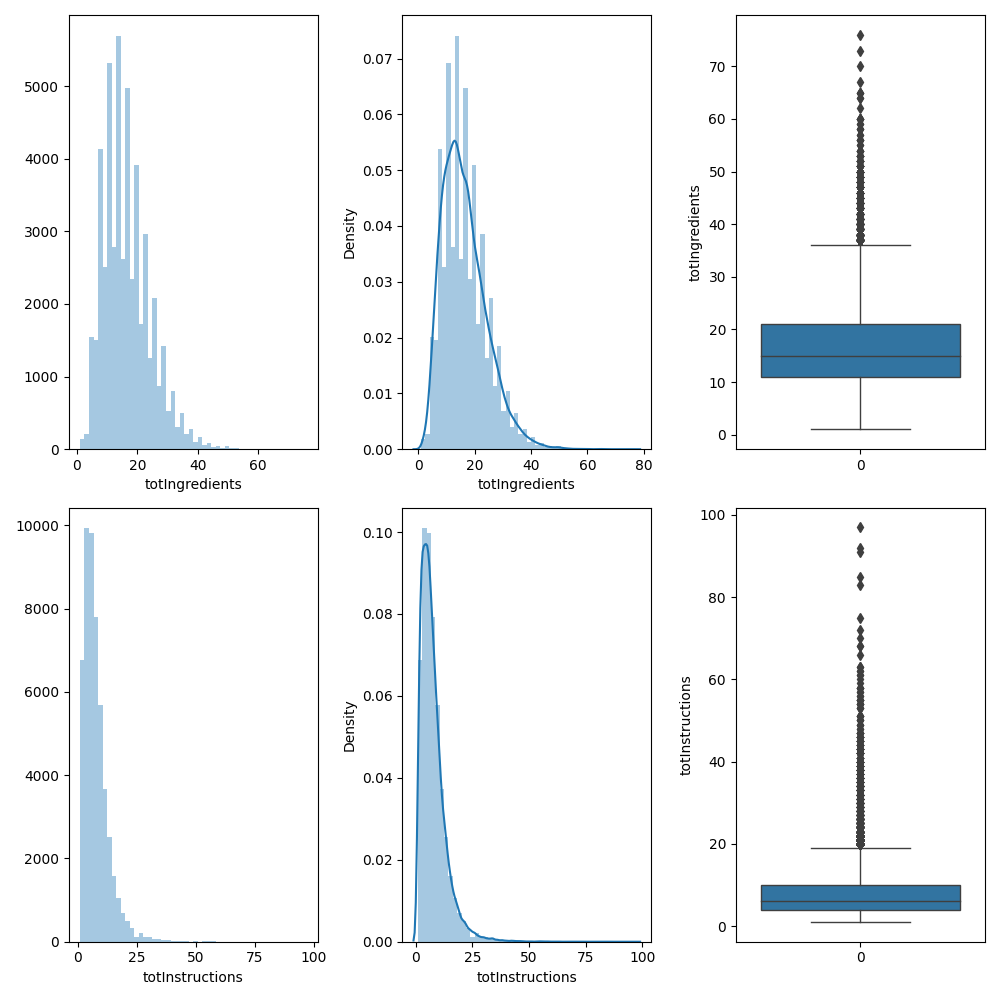
\includegraphics[width = 0.7 \linewidth]{images/displot.png}
    \centering
    \caption{Dstributions of lines per ingredients and instructions.}
    \label{distributions}
\end{figure}